\documentclass[11pt,letterpaper]{article}
\usepackage[T1]{fontenc}
\usepackage[scaled]{helvet}
\renewcommand{\familydefault}{\sfdefault}
\usepackage{amsmath,amssymb}
\usepackage[margin=0.8in,bottom=0.9in]{geometry}
\usepackage[most]{tcolorbox}
\usepackage{tikz}
\usetikzlibrary{calc}
\usepackage{enumitem}
\usepackage{array}
\usepackage{needspace}
\usepackage{fancyhdr}
\usepackage{pifont}

% ---- Palette "F. Bright & Playful" ----
\definecolor{fmtitle}{HTML}{3D2C8D}
\definecolor{fmkey}{HTML}{0096C7}
\definecolor{fmwatch}{HTML}{2BB673}
\definecolor{fmturn}{HTML}{F4A100}
\definecolor{fmmistake}{HTML}{EF476F}
\definecolor{fmnotice}{HTML}{9B5DE5}
\definecolor{fmgray}{HTML}{6B6B6B}

\pagestyle{fancy}
\fancyhf{}
\renewcommand{\headrulewidth}{0pt}
\fancyfoot[C]{\footnotesize\color{fmgray}\textcopyright\ 2026 FangMath. All rights reserved.}
\fancyfoot[R]{\footnotesize\color{fmgray}\thepage}
\setlength{\parindent}{0pt}
\setlength{\parskip}{3pt}

\newcommand{\badge}[1]{\colorbox{fmtitle}{\color{white}\bfseries\small\ #1\ }}
\newcommand{\leveltag}[2]{\colorbox{#1}{\color{white}\bfseries\scriptsize\ #2\ }}
\newcommand{\LE}{\leveltag{fmwatch}{EASY}}
\newcommand{\LM}{\leveltag{fmturn}{MEDIUM}}
\newcommand{\LH}{\leveltag{fmmistake}{HARD}}

\newcommand{\sectionbar}[2]{\needspace{6cm}\par\vspace{4mm}
  \begin{tcolorbox}[enhanced,colback=fmtitle,colframe=fmtitle,arc=2mm,
    left=4mm,top=1.5mm,bottom=1.5mm]
  \color{white}\bfseries\large #1\hfill{\normalsize\mdseries #2}
  \end{tcolorbox}}

\newtcolorbox{keyidea}{enhanced,breakable,colback=white,colframe=fmkey,boxrule=1pt,arc=2mm,
  title={Key Idea},coltitle=fmkey,fonttitle=\bfseries,
  attach boxed title to top left={xshift=4mm,yshift=-2mm},
  boxed title style={colback=white,colframe=fmkey,boxrule=0.9pt}}
\newtcolorbox{watchme}{enhanced,colback=white,colframe=fmwatch,boxrule=1pt,arc=2mm,
  title={Watch Me --- Worked Example},coltitle=fmwatch,fonttitle=\bfseries,
  attach boxed title to top left={xshift=4mm,yshift=-2mm},
  boxed title style={colback=white,colframe=fmwatch,boxrule=0.9pt}}
\newtcolorbox{mistakebox}{enhanced,breakable,colback=white,colframe=fmmistake,boxrule=1pt,arc=2mm,
  title={Common Mistake},coltitle=fmmistake,fonttitle=\bfseries,
  attach boxed title to top left={xshift=4mm,yshift=-2mm},
  boxed title style={colback=white,colframe=fmmistake,boxrule=0.9pt}}
\newtcolorbox{yourturn}{enhanced,breakable,colback=white,colframe=fmturn,boxrule=1pt,arc=2mm,
  title={Your Turn},coltitle=fmturn,fonttitle=\bfseries,
  attach boxed title to top left={xshift=4mm,yshift=-2mm},
  boxed title style={colback=white,colframe=fmturn,boxrule=0.9pt}}
\newtcolorbox{answerbox}[1]{enhanced,breakable,colback=white,colframe=fmwatch,boxrule=1pt,arc=2mm,
  title={#1},coltitle=fmwatch,fonttitle=\bfseries,
  attach boxed title to top left={xshift=4mm,yshift=-2mm},
  boxed title style={colback=white,colframe=fmwatch,boxrule=0.9pt}}

\newcommand{\work}[1]{\par\vspace{#1}}
\setlist[enumerate]{itemsep=2pt,topsep=3pt}

% ---------------- extra boxes ----------------
\newtcolorbox{notebox}{enhanced,breakable,colback=white,colframe=fmnotice,boxrule=1pt,arc=2mm,
  title={Notice},coltitle=fmnotice,fonttitle=\bfseries,
  attach boxed title to top left={xshift=4mm,yshift=-2mm},
  boxed title style={colback=white,colframe=fmnotice,boxrule=0.9pt}}
\newtcolorbox{exbox}{enhanced,colback=white,colframe=fmwatch,boxrule=0.8pt,arc=2mm,
  title={Example},coltitle=fmwatch,fonttitle=\bfseries\small,
  attach boxed title to top left={xshift=4mm,yshift=-2mm},
  boxed title style={colback=white,colframe=fmwatch,boxrule=0.8pt},fontupper=\small}
\newcommand{\topicbar}[1]{\needspace{4.5cm}\par\vspace{5mm}
  \begin{tcolorbox}[enhanced,colback=fmtitle,colframe=fmtitle,arc=2mm,left=4mm,top=1.5mm,bottom=1.5mm]
  \color{white}\bfseries\large #1
  \end{tcolorbox}}
\usepackage{multicol}

% ---------------- practice layout ----------------
\newcommand{\workline}{\par\vspace{7mm}{\color{gray!55}\rule{\linewidth}{0.4pt}}}
\newcommand{\worklines}[1]{\foreach \i in {1,...,#1}{\workline}}
\newcommand{\prob}[3]{\needspace{#3}\par\vspace{3mm}{\color{fmturn}\bfseries #1.}\ #2\par}
\newcommand{\ansline}{\par\vspace{4mm}\hfill\textbf{Answer:}\ \rule{5cm}{0.4pt}\par}
\newcommand{\keyitem}[3]{\needspace{3.2cm}\par\vspace{2mm}
  \begin{tcolorbox}[enhanced,colback=white,colframe=fmwatch!60,boxrule=0.6pt,arc=1.5mm,left=3mm,top=1.5mm,bottom=1.5mm]
  {\color{fmwatch}\bfseries #1.}\quad\small #2\par\vspace{1mm}
  \normalsize\textbf{Answer: #3}
  \end{tcolorbox}}


\usetikzlibrary{arrows.meta}
\providecommand{\iskey}{0}
% fill-in blank: line for students, pink answer in the key
\newcommand{\fb}[2][2.6cm]{\ifnum\iskey=1 \underline{\makebox[#1][c]{\color{fmmistake}\bfseries #2}}\else\underline{\makebox[#1]{}}\fi}
% answer line for practice problems
\newcommand{\pans}[2][3.2cm]{\ifnum\iskey=1 \underline{\makebox[#1][c]{\color{fmmistake}\bfseries #2}}\else\rule{#1}{0.4pt}\fi}
\newcommand{\vid}[1]{{\color{fmgray}\small\textit{\ding{43} Video: #1}}}
\newcommand{\pt}[2]{\fill (#1) circle (2.2pt) node[above=1pt,font=\small]{$#2$};}

\usetikzlibrary{decorations.pathreplacing}
\newcommand{\gridb}[4]{\draw[gray!30,step=1] (#1,#2) grid (#3,#4);\draw[gray!70,-{Stealth}] (#1,0)--(#3+0.4,0);\draw[gray!70,-{Stealth}] (0,#2)--(0,#4+0.4);}
\newcommand{\sdp}[3]{\begin{minipage}[t][2.4cm]{0.48\linewidth}{\color{fmturn}\bfseries #1.}\ #2\par\vfill\hfill \pans[3.6cm]{#3}\end{minipage}}
\newcommand{\sdpw}[3]{\begin{minipage}[t][2.4cm]{0.48\linewidth}{\color{fmturn}\bfseries #1.}\ #2\par\vfill\hfill \pans[5.2cm]{#3}\end{minipage}}
\newcommand{\algp}[3]{\begin{minipage}[t][4.2cm]{0.48\linewidth}{\color{fmturn}\bfseries #1.}\ #2\par\vfill\hfill \pans[4.4cm]{#3}\end{minipage}}
\newcommand{\pair}[2]{\needspace{3.4cm}\noindent #1\hfill #2\par\vspace{2mm}}
\newcommand{\head}[2]{\ifnum\iskey=1 \colorbox{fmwatch}{\color{white}\bfseries\small\ ANSWER KEY\ }\else\badge{#1}\fi\hfill{\small\color{fmgray}Geometry \textperiodcentered\ Lesson #2}\par\vspace{4mm}}
\newcommand{\nameline}{Name: \rule{6cm}{0.4pt}\hspace{1cm}Date: \rule{3.5cm}{0.4pt}\par\vspace{2mm}}
\renewcommand{\vid}[1]{\needspace{4.2cm}{\color{fmgray}\small\textit{\ding{43} Video: #1}}}
\begin{document}
\head{WATCH \& FILL IN}{1.5}
{\color{fmtitle}\LARGE\bfseries Angles --- Notes\ifnum\iskey=1 \ --- Answer Key\fi}\par\vspace{1mm}
{\color{fmgray}Watch the video and fill in each blank. Pause when you see ``Your turn.''}\par\vspace{3mm}
\nameline

\vid{Four kinds of angles}
\begin{keyidea}\begin{tabular}{@{}>{\centering\arraybackslash}p{0.22\linewidth}>{\centering\arraybackslash}p{0.22\linewidth}>{\centering\arraybackslash}p{0.22\linewidth}>{\centering\arraybackslash}p{0.22\linewidth}@{}}
\tikz{\draw[thick,-{Stealth}] (0,0)--(1.4,0);\draw[thick,-{Stealth}] (0,0)--(55:1.4);\draw[fmkey] (0.4,0) arc (0:55:0.4);} &
\tikz{\draw[thick,-{Stealth}] (0,0)--(1.4,0);\draw[thick,-{Stealth}] (0,0)--(0,1.4);\draw[fmkey] (0.3,0)--(0.3,0.3)--(0,0.3);} &
\tikz{\draw[thick,-{Stealth}] (0,0)--(1.4,0);\draw[thick,-{Stealth}] (0,0)--(130:1.4);\draw[fmkey] (0.4,0) arc (0:130:0.4);} &
\tikz{\draw[thick,{Stealth}-{Stealth}] (-1,0)--(1,0);\fill (0,0) circle(2pt);\draw[fmkey] (0.35,0) arc (0:180:0.35);\path (0,1.1);}\\
\textbf{Acute} & \textbf{Right} & \textbf{Obtuse} & \textbf{Straight}\\
\fb[2.6cm]{less than $90^\circ$} & \fb[2.6cm]{exactly $90^\circ$} & between $90^\circ$ and \fb[1.2cm]{$180^\circ$} & \fb[2.6cm]{exactly $180^\circ$}\\
\end{tabular}\end{keyidea}

\vid{Reading an angle's name}
\begin{keyidea}In $\angle ABD$, the vertex is the \fb[1.6cm]{middle} letter: \fb[0.8cm]{$B$}. \quad $\angle ABD$ and $\angle DBA$ name the \fb[1.4cm]{same} angle.\end{keyidea}

\vid{Angle Addition Postulate}
\begin{keyidea}\begin{minipage}[c]{0.32\linewidth}\centering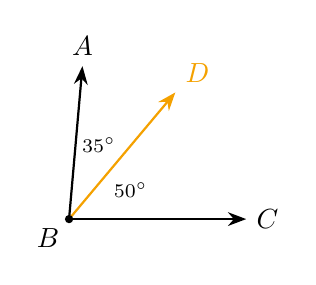
\begin{tikzpicture}[scale=0.75]
\draw[thick,-{Stealth}] (0,0)--(3,0) node[right]{$C$};\draw[thick,-{Stealth}] (0,0)--(85:2.6) node[above]{$A$};\draw[thick,-{Stealth},fmturn] (0,0)--(50:2.8) node[above right]{$D$};
\fill (0,0) circle(2pt) node[below left]{$B$};\node[font=\scriptsize] at (25:1.15){$50^\circ$};\node[font=\scriptsize] at (68:1.35){$35^\circ$};\end{tikzpicture}\end{minipage}\hfill
\begin{minipage}[c]{0.64\linewidth}$D$ is inside $\angle ABC$. \ $m\angle ABD = 35^\circ$, \ $m\angle DBC = 50^\circ$.\par\vspace{1mm}
$m\angle ABC = 35 + 50 = $ \fb[1.4cm]{$85^\circ$} \ --- the small angles \fb[1.4cm]{add} to the big one.\par\vspace{1mm}
$85^\circ < 90^\circ$, so it is \fb[1.6cm]{acute}.\end{minipage}\end{keyidea}

\vid{With algebra}
\begin{watchme}$D$ is inside $\angle ABC$. \ $m\angle ABD = 2x + 5$, \ $m\angle DBC = 3x$, \ $m\angle ABC = 80^\circ$. Find $m\angle DBC$.\par\vspace{2mm}
$(2x + 5) + 3x = 80$ \ (part $+$ part $=$ whole) \quad $\Rightarrow$ \quad $5x + 5 = 80$ \quad $\Rightarrow$ \quad $x = $ \fb[1.1cm]{$15$}\par\vspace{1mm}
$m\angle DBC = 3(15) = $ \fb[1.4cm]{$45^\circ$} \qquad Check: $35 + 45 = 80$ \ding{51}\end{watchme}

\vid{Angle pairs}
\begin{keyidea}\textbf{Complementary} angles add to \fb[1.4cm]{$90^\circ$}. \quad \textbf{Supplementary} angles add to \fb[1.4cm]{$180^\circ$}.\par\vspace{1mm}
{\small Memory trick: \textbf{C} comes before \textbf{S} in the alphabet --- just like $90$ comes before $180$.}\par\vspace{2mm}
Supplement of $65^\circ$: $180 - 65 = $ \fb[1.4cm]{$115^\circ$} \qquad Complement of $65^\circ$: $90 - 65 = $ \fb[1.4cm]{$25^\circ$}\end{keyidea}

\vid{Vertical angles and linear pairs}
\begin{keyidea}\begin{minipage}[c]{0.3\linewidth}\centering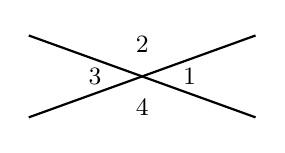
\begin{tikzpicture}[scale=0.8]
\draw[thick] (-1.8,-0.65)--(1.8,0.65);\draw[thick] (-1.8,0.65)--(1.8,-0.65);
\node[font=\small] at (0.75,0){$1$};\node[font=\small] at (0,0.5){$2$};\node[font=\small] at (-0.75,0){$3$};\node[font=\small] at (0,-0.5){$4$};\end{tikzpicture}\end{minipage}\hfill
\begin{minipage}[c]{0.66\linewidth}\textbf{Vertical angles} are across from each other and are \fb[1.4cm]{equal}: $\angle 1 = \angle 3$.\par\vspace{1mm}
A \textbf{linear pair} is side by side on a line and adds to \fb[1.4cm]{$180^\circ$}.\par\vspace{1mm}
If $\angle 1 = 40^\circ$: \ $\angle 3 = $ \fb[1.2cm]{$40^\circ$}, \ $\angle 2 = \angle 4 = $ \fb[1.4cm]{$140^\circ$}\end{minipage}\end{keyidea}

\vid{Your turn}
\begin{yourturn}$\angle 1$ and $\angle 2$ are supplementary. $m\angle 1 = 4x + 20$, \ $m\angle 2 = 2x + 40$. Find $x$ and both angles.\par\vspace{2mm}
$(4x + 20) + (2x + 40) = 180$ \quad $\Rightarrow$ \quad $6x + 60 = 180$ \quad $\Rightarrow$ \quad $x = $ \fb[1.1cm]{$20$}\par\vspace{1mm}
$m\angle 1 = $ \fb[1.4cm]{$100^\circ$}, \quad $m\angle 2 = $ \fb[1.4cm]{$80^\circ$}\end{yourturn}
\end{document}
